\documentclass[letterpaper]{article}
\usepackage{natbib}
\usepackage[utf8]{inputenc}
\usepackage{graphicx}
\usepackage{color}
\usepackage{multirow}
\usepackage{amsmath}
\usepackage{array}
\usepackage{subcaption}
\usepackage{mathpazo}
\usepackage[a4paper]{geometry}
\usepackage{float}

\title{Learning Dynamics: Assignment 3 \\
\Large Multi-Armed Bandits}
\author{\Large Hakim Boulahya \\ \\
Université Libre de Bruxelles \\
hboulahy@ulb.ac.be - 000391737
}

\begin{document}
\maketitle
\tableofcontents
\newpage

\section{N-Armed Bandit}


\subsection{Exercice 1}

% ex1 rewards
\begin{figure}[H]
    \centering
    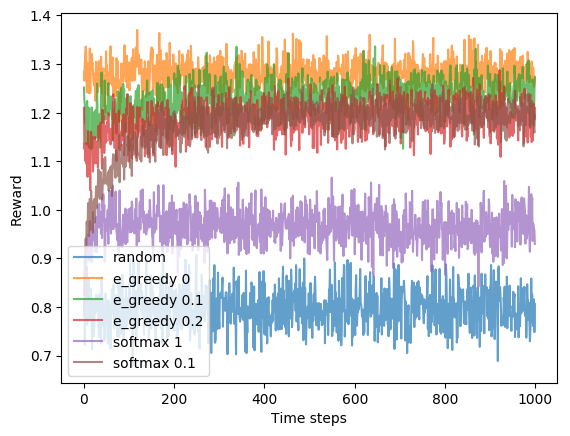
\includegraphics[width=.7\linewidth]{images/assign3/ex1/rewards}
    \caption{Average rewards for all algorithms}
    \label{fig:rewards_ex1}
\end{figure}

We can see that only exploring \textit{i.e.} doesn't perform well, and
the reward stay low. The boltzmann distribution of softmax with a temparature
of 1 also has a poor performance compared to the other methods. Using softmax
with a temparature of 0.1 gives better results. Using e-greedy with small
value, i.e. will likely choose the action with the best optimum, tends
to better results. egreedy with 0 seems to arrives
\textit{directly} to the best arm. We can see on the graph that when $\epsilon$
is bigger it usually takes more time to get to the best arm.
Softmax with a temperature of 0.1 does tends to the best arm, but takes more
time.

% ex1 qtas
\begin{figure}[H]
  \begin{subfigure}{.5\textwidth}
    \centering
    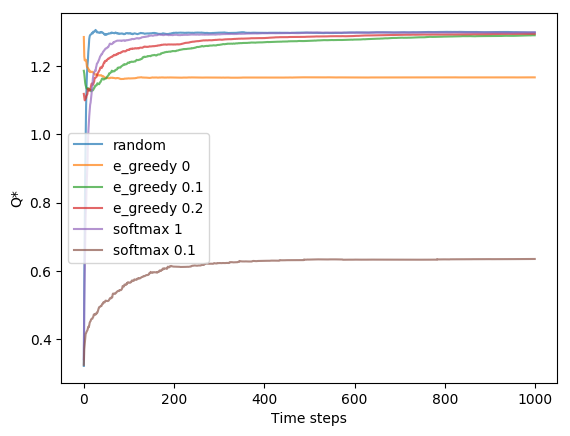
\includegraphics[width=1\linewidth]{images/assign3/ex1/qta_0}
    \caption{$Q_{a_{0}}(t)$}
    \label{fig:qta_0_ex1}
  \end{subfigure}
  \begin{subfigure}{.5\textwidth}
    \centering
    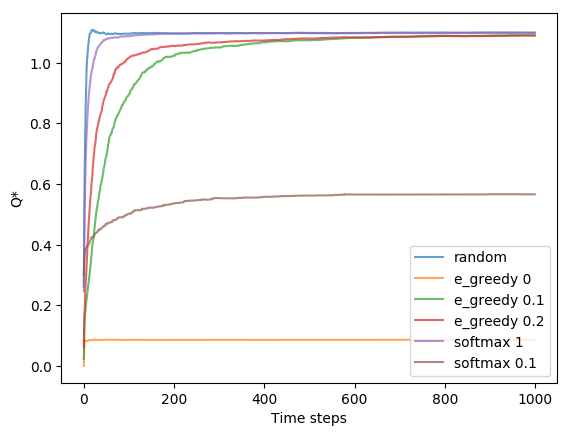
\includegraphics[width=1\linewidth]{images/assign3/ex1/qta_1}
    \caption{$Q_{a_{1}}(t)$}
    \label{fig:qta_1_ex1}
  \end{subfigure}
  \begin{subfigure}{.5\textwidth}
    \centering
    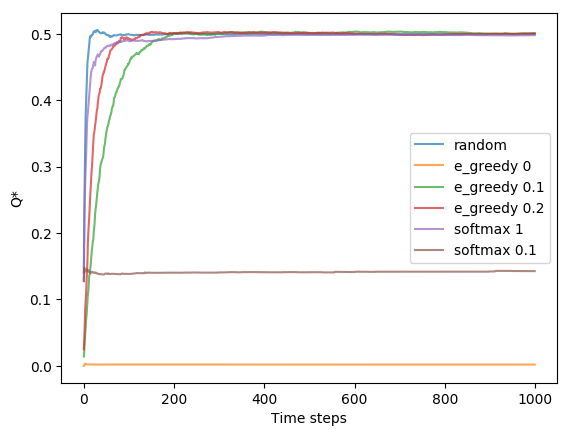
\includegraphics[width=1\linewidth]{images/assign3/ex1/qta_2}
    \caption{$Q_{a_{2}}(t)$}
    \label{fig:qta_2_ex1}
  \end{subfigure}
  \begin{subfigure}{.5\textwidth}
    \centering
    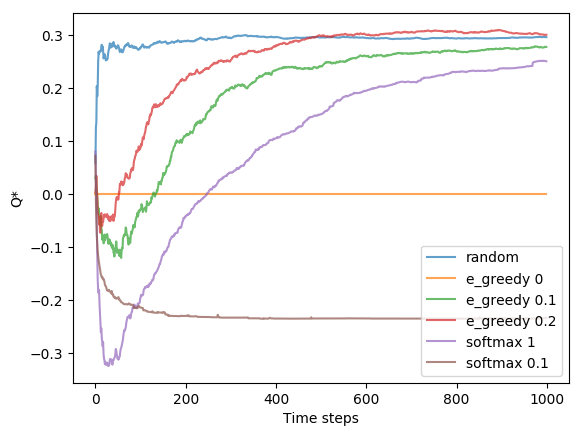
\includegraphics[width=1\linewidth]{images/assign3/ex1/qta_3}
    \caption{$Q_{a_{3}}(t)$}
    \label{fig:qta_3_ex1}
  \end{subfigure}

    \caption{Plot per arm showing
    the $Q^{*}_{a_{i}}$
    of that action along with the actual $Q_{a_{i}}$ a i estimate over time
    with
    $\mu$ = (1.3, 1.1, 0.5, 0.3), $\sigma$ = (0.9, 0.6, 0.4, 2.0)}
    \label{fig:qtas_ex1}
\end{figure}

\paragraph{egreedy 0}

Since the algorithm will always choose the optimum $Q^*$, we can see on
Figure \ref{fig:qtas_ex1} that the player never explore, i.e. it has
no estimation of the Q-values, except for for the best $Q^*$, which is
$Q*a1$

\paragraph{random}

Since the random methods chooses all actions with the same count, the player
will explore the environment, therefore will be able to determine all
Q-values to be close enough to the optimum.


% EX1 arms histograms
\begin{figure}[H]
  \begin{subfigure}{.5\textwidth}
    \centering
    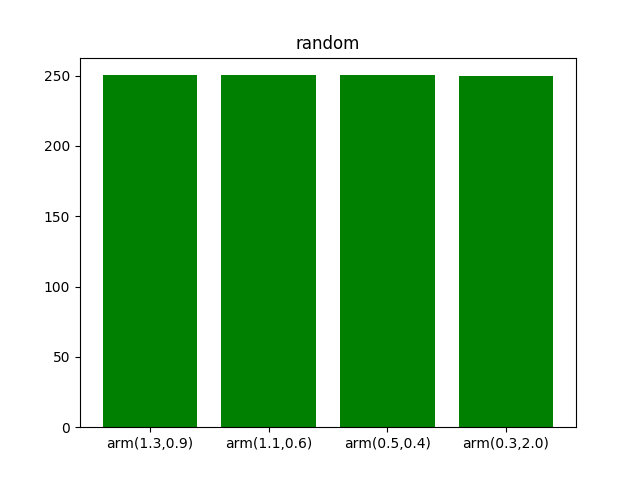
\includegraphics[width=1\linewidth]{images/assign3/ex1/arms_random}
    \caption{}
    \label{fig:arms_random_ex1}
  \end{subfigure}
  \begin{subfigure}{.5\textwidth}
    \centering
    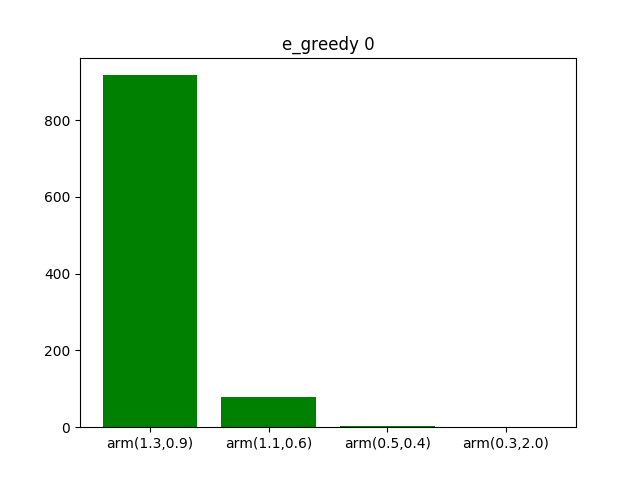
\includegraphics[width=1\linewidth]{images/assign3/ex1/arms_e_greedy0}
    \caption{}
    \label{fig:arms_e_greedy0_ex1}
  \end{subfigure}
  \begin{subfigure}{.5\textwidth}
    \centering
    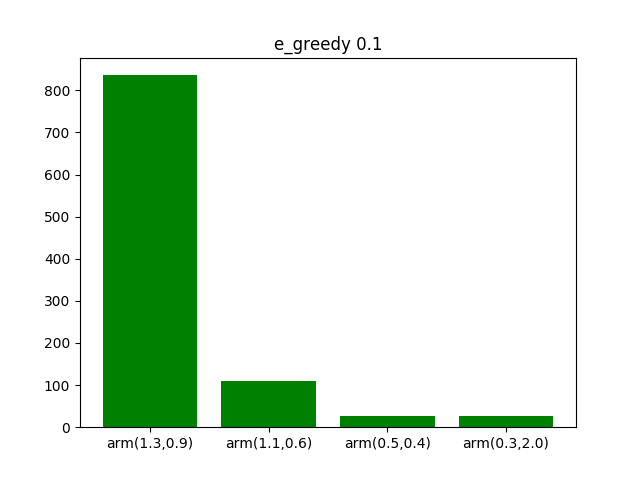
\includegraphics[width=1\linewidth]{images/assign3/ex1/arms_e_greedy01}
    \caption{}
    \label{fig:arms_e_greedy01_ex1}
  \end{subfigure}
  \begin{subfigure}{.5\textwidth}
    \centering
    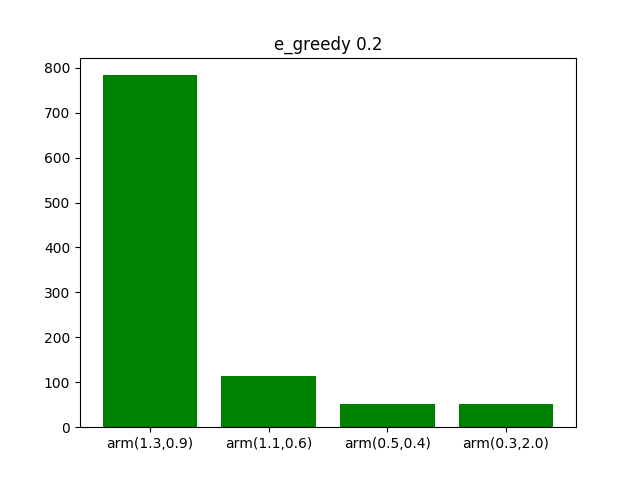
\includegraphics[width=1\linewidth]{images/assign3/ex1/arms_e_greedy02}
    \caption{}
    \label{fig:arms_e_greedy02_ex1}
  \end{subfigure}
  \begin{subfigure}{.5\textwidth}
    \centering
    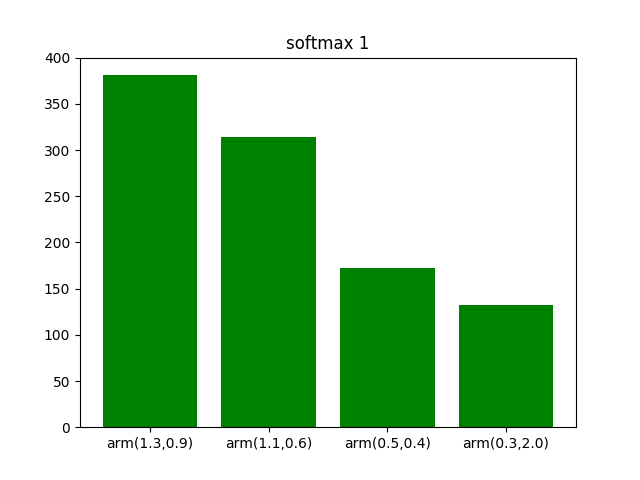
\includegraphics[width=1\linewidth]{images/assign3/ex1/arms_softmax1}
    \caption{}
    \label{fig:arms_softmax1_ex1}
  \end{subfigure}
  \begin{subfigure}{.5\textwidth}
    \centering
    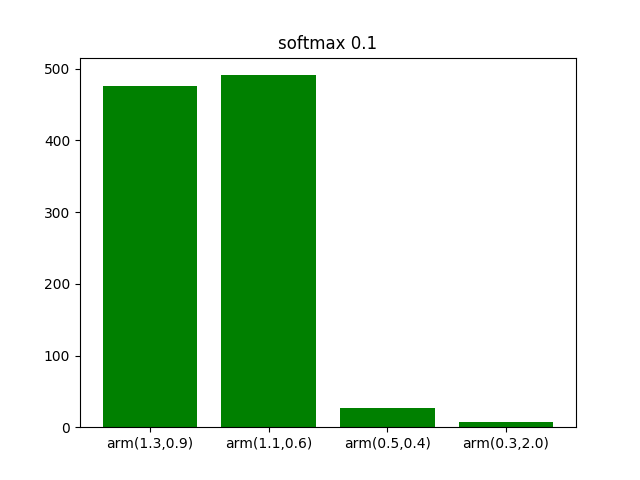
\includegraphics[width=1\linewidth]{images/assign3/ex1/arms_softmax01}
    \caption{}
    \label{fig:arms_softmax01_ex1}
  \end{subfigure}
    \caption{Histograms showing the number of times each action is selected
    per selection strategy with
    $\mu$ = (1.3, 1.1, 0.5, 0.3), $\sigma$ = (0.9, 0.6, 0.4, 2.0)}
    \label{fig:arms_ex1}
\end{figure}

\paragraph{Random}

The random chooses the action based on uniform distribution. So it is
logical chooses all arms the same count.

e-greedy methods tends to follow the same pattern. The best arm is chosen
most of the time. It is due to the fact that $\epsilon$ is small, which
mean that the probability to choose the biggest optimum is more important.
We can see that more \epsilon is greather, more the histograms shows that
non-optimal arms are chosen.


\subsection{Exercice 2}

% ex2 rewards
\begin{figure}[H]
    \centering
    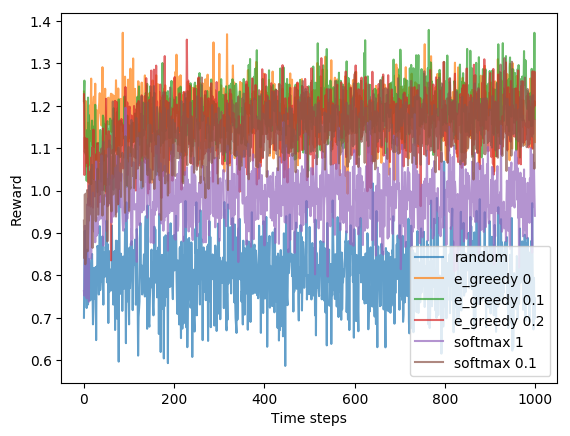
\includegraphics[width=.7\linewidth]{images/assign3/ex2/rewards}
    \caption{Average rewards for all algorithms}
    \label{fig:rewards_ex2}
\end{figure}

The results order of the algorithm that perform best doesn't really changes.
By doubling the standard deviation, we only allowed the algorithms to
provide a more random rewards \textit{i.e.} a bigger range. We can see
that the dynamics of the algorithms don't change.


It is harder to learn because of the standard deviation that provides
ar more randomize outcomes, therefore harder to find the best reward.

% ex2 qtas
\begin{figure}[H]
  \begin{subfigure}{.5\textwidth}
    \centering
    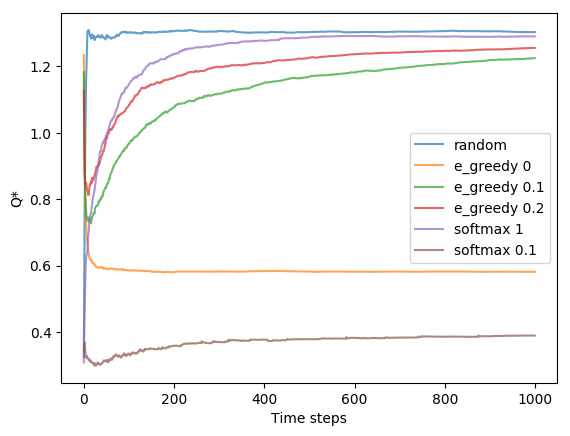
\includegraphics[width=1\linewidth]{images/assign3/ex2/qta_0}
    \caption{$Q_{a_{0}}(t)$}
    \label{fig:qta_0_ex2}
  \end{subfigure}
  \begin{subfigure}{.5\textwidth}
    \centering
    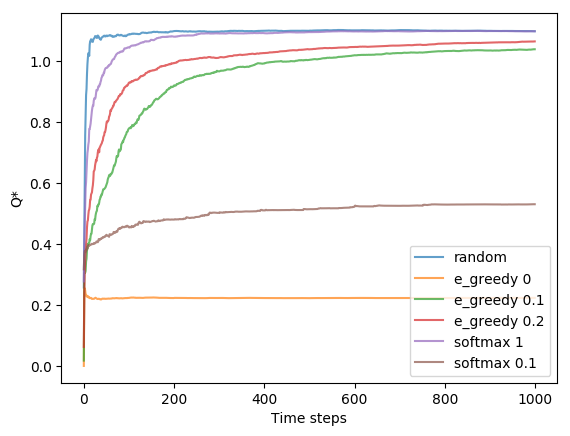
\includegraphics[width=1\linewidth]{images/assign3/ex2/qta_1}
    \caption{$Q_{a_{1}}(t)$}
    \label{fig:qta_1_ex2}
  \end{subfigure}
  \begin{subfigure}{.5\textwidth}
    \centering
    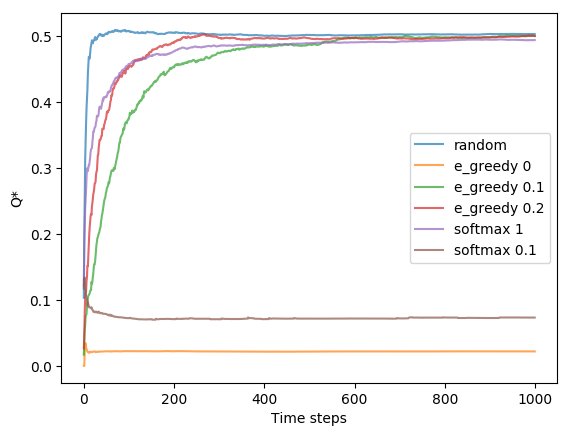
\includegraphics[width=1\linewidth]{images/assign3/ex2/qta_2}
    \caption{$Q_{a_{2}}(t)$}
    \label{fig:qta_2_ex2}
  \end{subfigure}
  \begin{subfigure}{.5\textwidth}
    \centering
    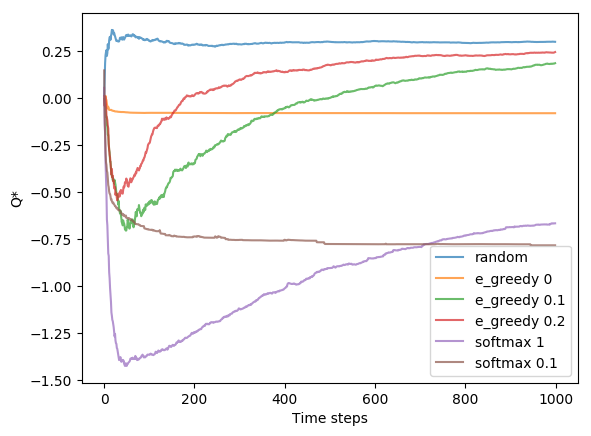
\includegraphics[width=1\linewidth]{images/assign3/ex2/qta_3}
    \caption{$Q_{a_{3}}(t)$}
    \label{fig:qta_3_ex2}
  \end{subfigure}

    \caption{Plot per arm showing
    the $Q^{*}_{a_{i}}$
    of that action along with the actual $Q_{a_{i}}$ a i estimate over time
    with
    $\mu$ = (1.3, 1.1, 0.5, 0.3), $\sigma$ = (1.8, 1.2, 0.8, 4.0)}
    \label{fig:qtas_ex2}
\end{figure}

% ex2 arms histograms
\begin{figure}[H]
  \begin{subfigure}{.5\textwidth}
    \centering
    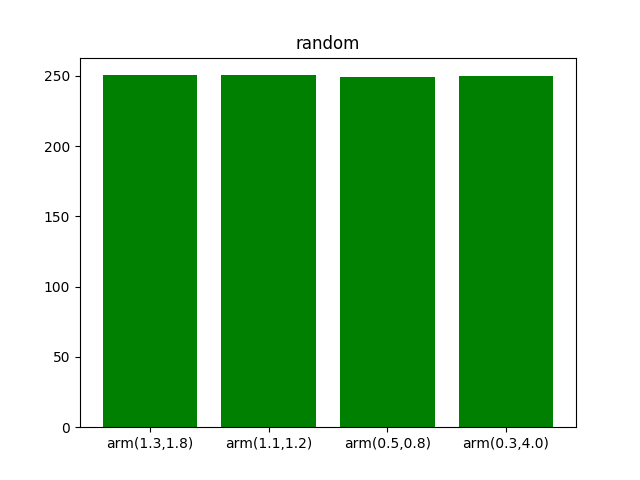
\includegraphics[width=1\linewidth]{images/assign3/ex2/arms_random}
    \caption{}
    \label{fig:arms_random_ex2}
  \end{subfigure}
  \begin{subfigure}{.5\textwidth}
    \centering
    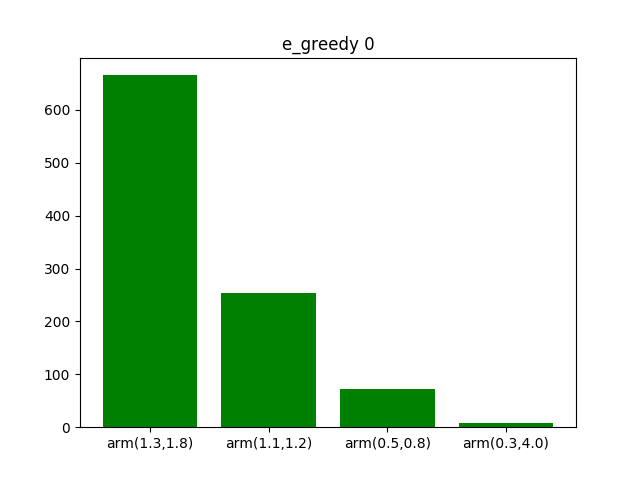
\includegraphics[width=1\linewidth]{images/assign3/ex2/arms_e_greedy0}
    \caption{}
    \label{fig:arms_e_greedy0_ex2}
  \end{subfigure}
  \begin{subfigure}{.5\textwidth}
    \centering
    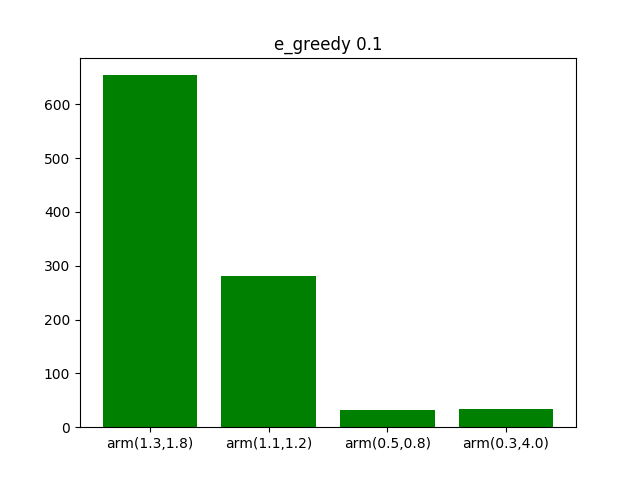
\includegraphics[width=1\linewidth]{images/assign3/ex2/arms_e_greedy01}
    \caption{}
    \label{fig:arms_e_greedy01_ex2}
  \end{subfigure}
  \begin{subfigure}{.5\textwidth}
    \centering
    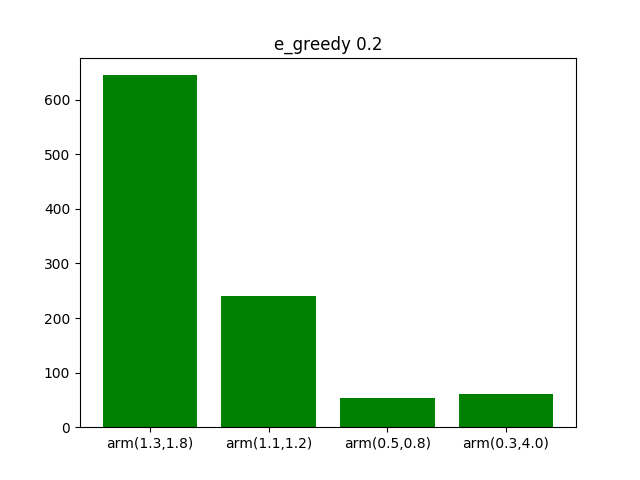
\includegraphics[width=1\linewidth]{images/assign3/ex2/arms_e_greedy02}
    \caption{}
    \label{fig:arms_e_greedy02_ex2}
  \end{subfigure}
  \begin{subfigure}{.5\textwidth}
    \centering
    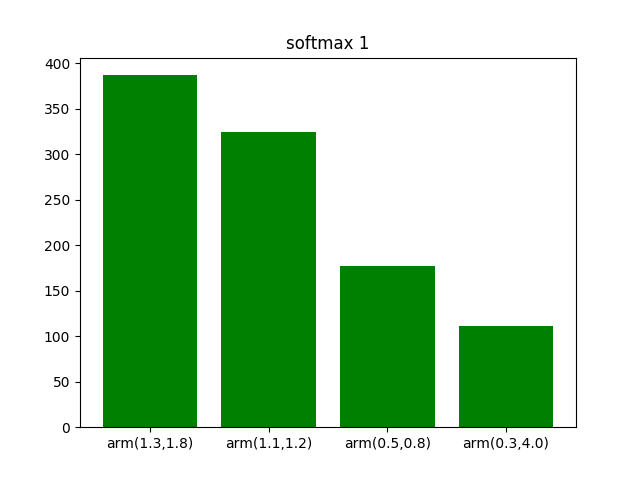
\includegraphics[width=1\linewidth]{images/assign3/ex2/arms_softmax1}
    \caption{}
    \label{fig:arms_softmax1_ex2}
  \end{subfigure}
  \begin{subfigure}{.5\textwidth}
    \centering
    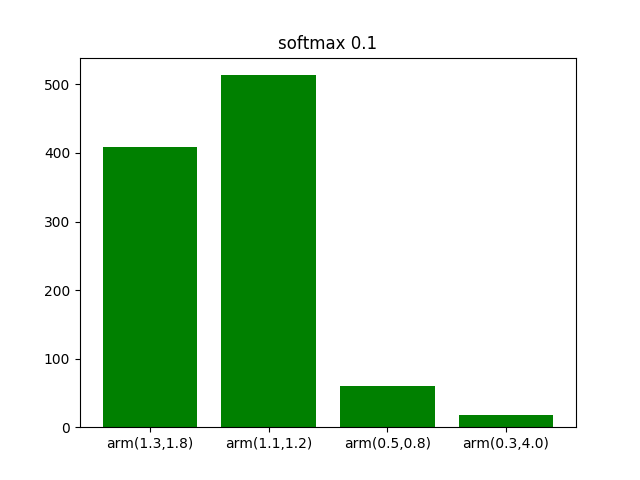
\includegraphics[width=1\linewidth]{images/assign3/ex2/arms_softmax01}
    \caption{}
    \label{fig:arms_softmax01_ex2}
  \end{subfigure}
    \caption{Histograms showing the number of times each action is selected
    per selection strategy with
    $\mu$ = (1.3, 1.1, 0.5, 0.3), $\sigma$ = (1.8, 1.2, 0.8, 4.0)}
    \label{fig:arms_ex2}
\end{figure}

The standard deviation is bigger, therefore the algorithms takes more time
to find the best arm.

\subsection{Exercice 3}

% ex3 rewards
\begin{figure}[H]
    \centering
    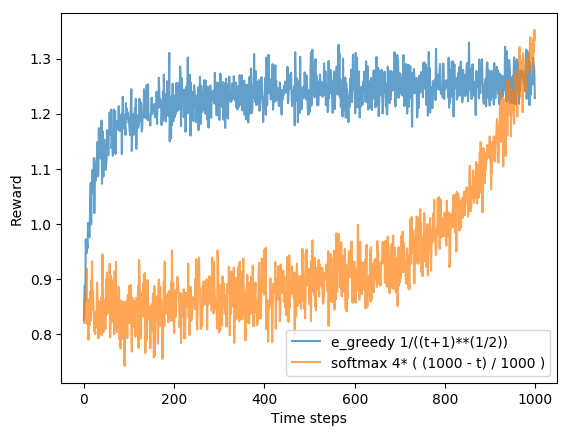
\includegraphics[width=.7\linewidth]{images/assign3/ex3/rewards}
    \caption{Average rewards for all algorithms}
    \label{fig:rewards_ex3}
\end{figure}

Dynamic egreedy doesn't seems to perform better that the statics one,
the resulting rewards tends to be identical. Observing the graph shows
us that it takes more time to stabilize to the best arm.

Dynamic softmax seems to be better, if you consider to long term reward.
It takes to the 1000 epoch for the algorithm to find the best arm in
opposition to the softmax using a a temperature of 0.1, where it
is close to the best arm at around epoch 200, but not as close as
the dynamic softmax, where it is closer to the best arm, when it
is stabilized.

% ex3 qtas
\begin{figure}[H]
  \begin{subfigure}{.5\textwidth}
    \centering
    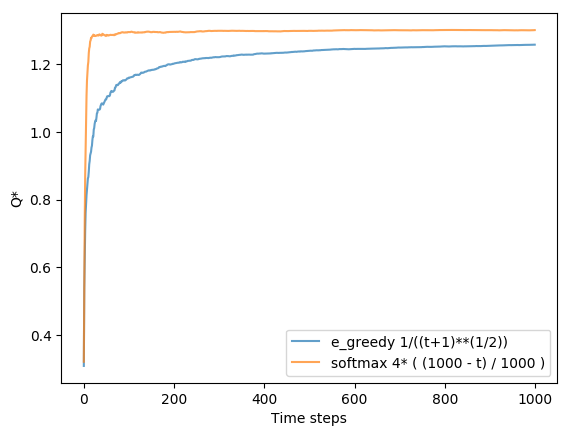
\includegraphics[width=1\linewidth]{images/assign3/ex3/qta_0}
    \caption{$Q_{a_{0}}(t)$}
    \label{fig:qta_0_ex3}
  \end{subfigure}
  \begin{subfigure}{.5\textwidth}
    \centering
    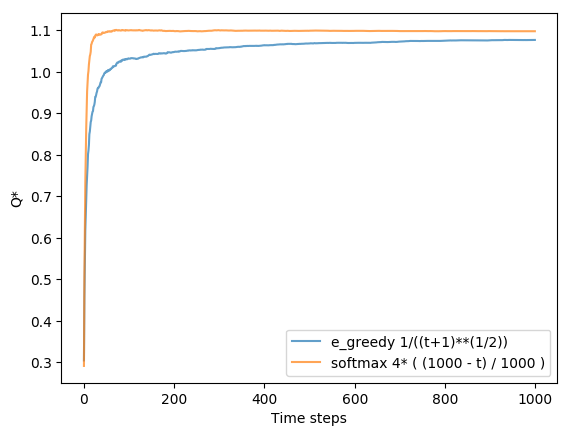
\includegraphics[width=1\linewidth]{images/assign3/ex3/qta_1}
    \caption{$Q_{a_{1}}(t)$}
    \label{fig:qta_1_ex3}
  \end{subfigure}
  \begin{subfigure}{.5\textwidth}
    \centering
    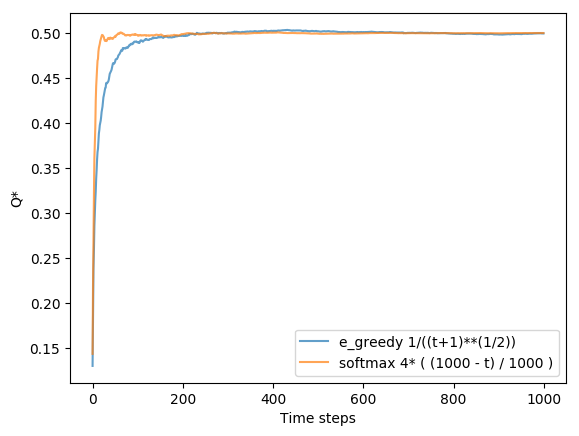
\includegraphics[width=1\linewidth]{images/assign3/ex3/qta_2}
    \caption{$Q_{a_{2}}(t)$}
    \label{fig:qta_2_ex3}
  \end{subfigure}
  \begin{subfigure}{.5\textwidth}
    \centering
    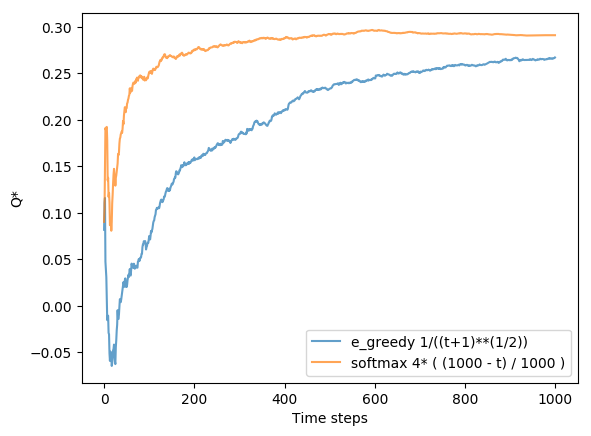
\includegraphics[width=1\linewidth]{images/assign3/ex3/qta_3}
    \caption{$Q_{a_{3}}(t)$}
    \label{fig:qta_3_ex3}
  \end{subfigure}

    \caption{Plot per arm showing
    the $Q^{*}_{a_{i}}$
    of that action along with the actual $Q_{a_{i}}$ a i estimate over time}
    \label{fig:qtas_ex3}
\end{figure}

% ex3 arms histograms
\begin{figure}[H]
    \begin{subfigure}{.5\textwidth}
    \centering
    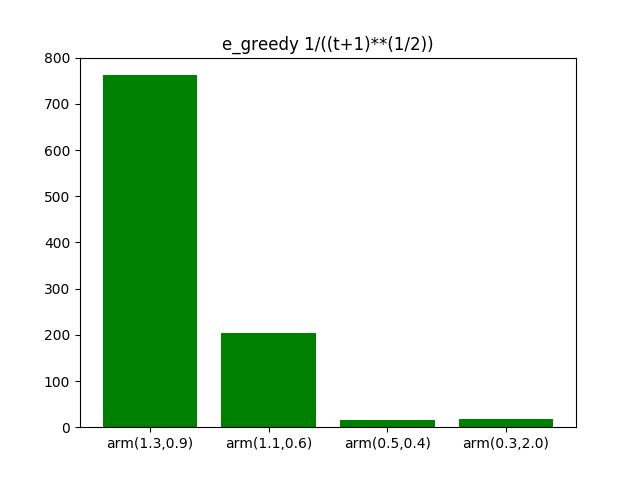
\includegraphics[width=1\linewidth]{images/assign3/ex3/arms_e_greedy_t}
    \caption{}
    \label{fig:arms_e_greedy_t_ex3}
    \end{subfigure}
    \begin{subfigure}{.5\textwidth}
      \centering
      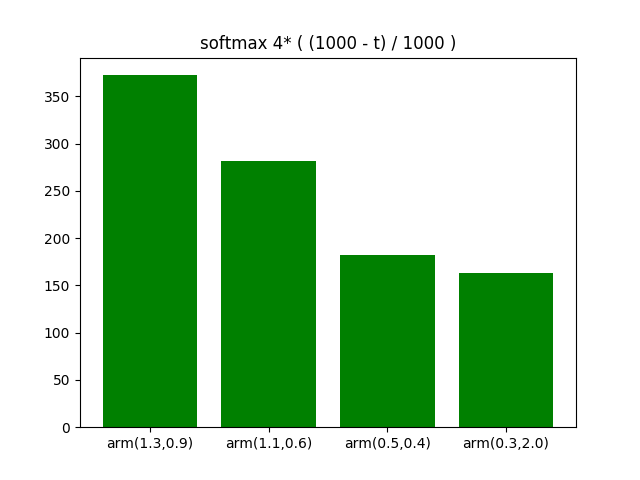
\includegraphics[width=1\linewidth]{images/assign3/ex3/arms_softmax_t}
      \caption{}
      \label{fig:arms_softmax_t_ex3}
    \end{subfigure}
    \caption{Histograms showing the number of times each action is selected
    per selection strategy}
    \label{fig:arms_ex3}
\end{figure}

\section{Climbing game}

When using the formula, it is important to have a big tau, because exp(Q/tau)
will give errors if Q is too big. (See how EV(a) is calculated)

I also remarked that when using EV with max_rewards or max_q when
min_tau = 0.001 the 11 is good, but when 0.1 or 1, not. THis is probably
due to the stochastic of our game.

\end{document}
